\documentclass[a4paper]{article}

\usepackage{amsmath, amssymb}
\usepackage{graphicx}
\usepackage{float}

\title{Project report}

\author{}

\begin{document}
\maketitle

\section{Solutions}
\begin{figure}[H]
	\centering
	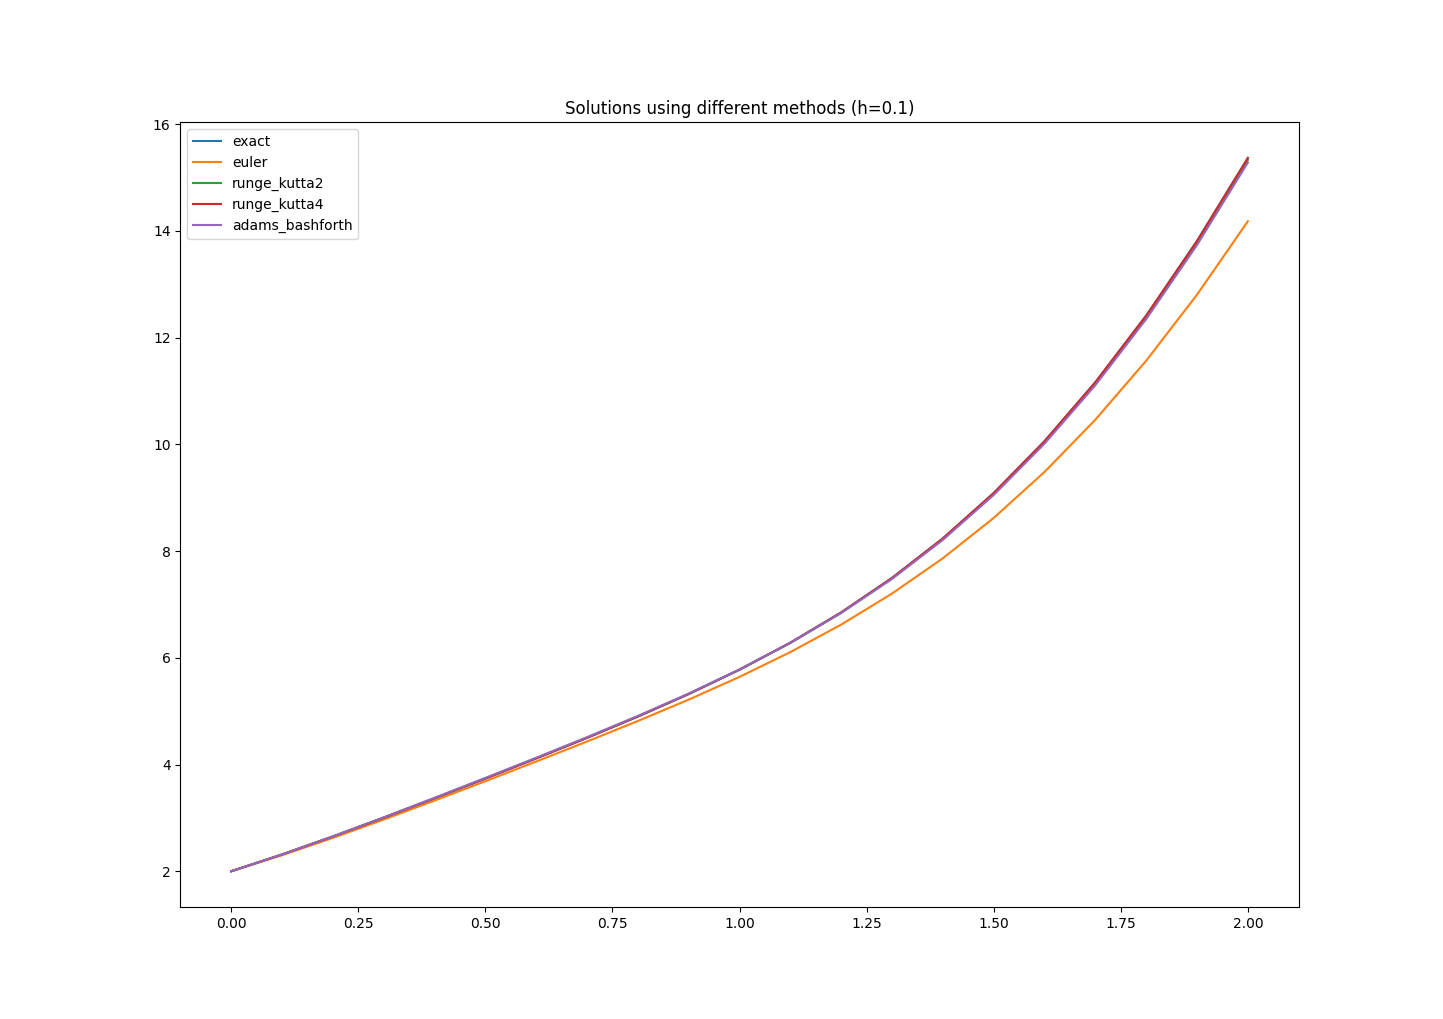
\includegraphics[width=\linewidth]{solutions.png}
\end{figure}

\section{Errors}
\begin{figure}[H]
	\centering
	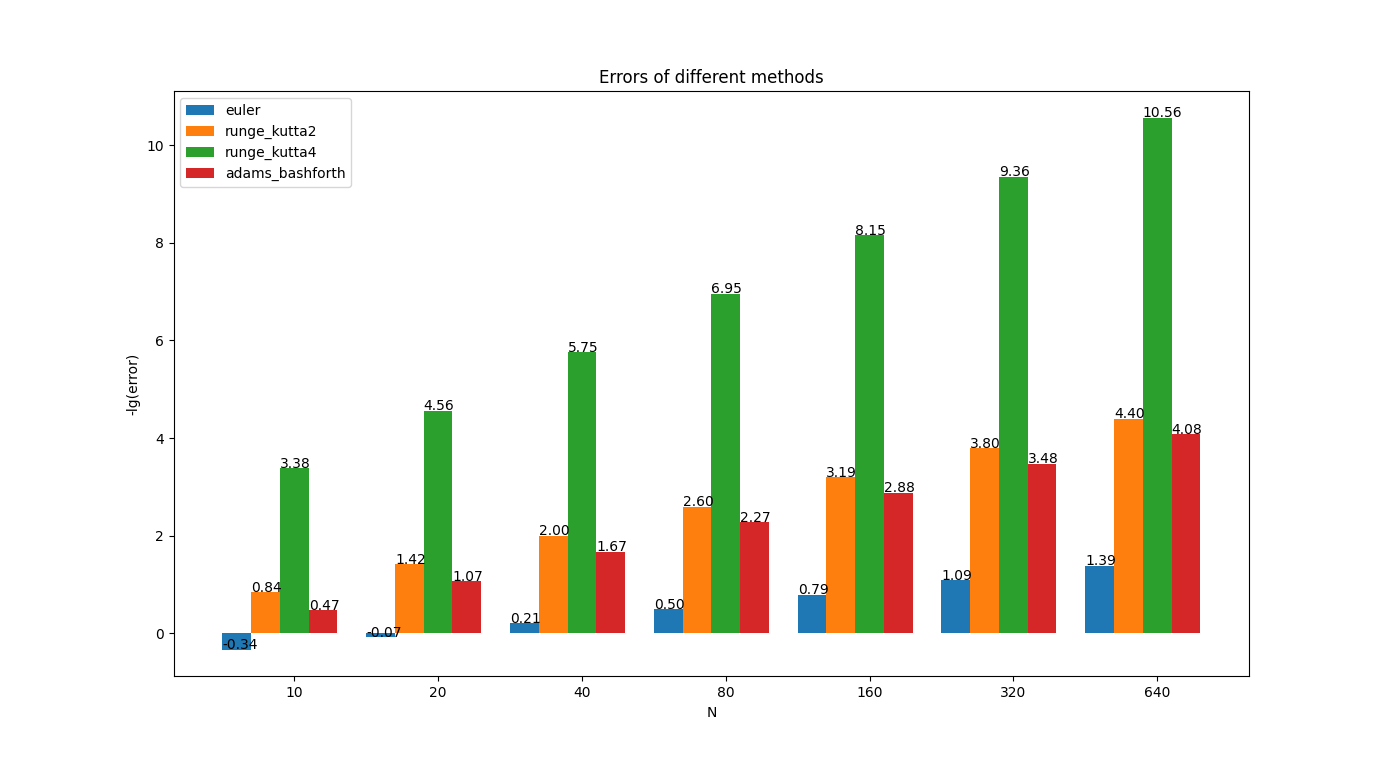
\includegraphics[width=\linewidth]{errors.png}
\end{figure}

Note that the y axis of the plot is $-\log(\epsilon)$ where
$\epsilon$ is the error. Hence the higher the bar is, the smaller
the error is. The reasoning is that most of the errors are very small (well
below 1), and using a logarithm plot is easier to find out the order of the
errors.

Forth order Runge-Kutta has the highest order. Second order Runge-Kutta has
similar order as Adams-Bashforth. Euler's method has the lowest order. Forth
order Runge-Kutta method performed the btest.

\end{document}
